\documentclass[UTF8]{ctexart}
\usepackage[backend=bibtex]{biblatex}
\usepackage[a4paper]{geometry}
\usepackage{fancyhdr}
\usepackage{appendix}
\usepackage{graphicx}
\usepackage{minted}
\usepackage{eqlist}
\usepackage{hyperref}
\usepackage{ulem}
\usepackage{CJKulem}
\usepackage[bottom]{footmisc}

\ctexset{secnumdepth=4,tocdepth=4}

\hypersetup{hidelinks,
	colorlinks=true,
	allcolors=black,
	pdfstartview=Fit,
	breaklinks=true}
\geometry{left=2.54cm,right=2.54cm,top=3.09cm,bottom=3.09cm}

\pagestyle{fancy}
\fancyhead{}
\fancyfoot{}
\fancyhead[L]{2023 程序设计 \uppercase\expandafter{\romannumeral2} 大作业:不围棋}
\fancyhead[R]{第二阶段报告}
\fancyfoot[C]{\thepage}

\title{2023 程序设计 \uppercase\expandafter{\romannumeral2} 大作业:不围棋\\第二阶段报告}
\author{彭文博、李知非、魏子洪}
\date{\today}
\begin{document}
\maketitle
\newpage
\tableofcontents
\newpage
\section{总览}
在第二阶段,我们主要致力于联机功能的开发。
由于我们先前采取了网络部分与游戏逻辑部分分离的架构设计,在本阶段我们只需在网络部分实现相应的 Operation 就可以实现联机游戏的核心功能。
目前我们的联机游戏功能上不仅达到了第二阶段的基本要求(不显式区分服务器和客户端、可自定义联机端口等),
还完成了*附加任务3*和*附加任务4*中对联机游戏的附加要求(支持再来一局、支持同时处理多个对局申请等),
并且具有完善和健全的联机逻辑,以及用户友好的联机游戏界面。
\par 在游戏逻辑方面,我们实现了本阶段要求的大部分功能,包括:
\begin{itemize} 
	\item 显示剩余时间、对局状态等信息
	\item 高亮标记最新落子的位置
	\item 红色警示必输的落子选择
	\item 对局结束后显示胜负结果和得分情况
\end{itemize}
\par
关于对局记录的保存和复现,我们计划在第三阶段中实现这一功能,并与*附加任务1*和*附加任务2*进行整合。
\par
我们正在积极开发多路棋盘功能。考虑到本项目优秀的架构设计,我们预估实现多路棋盘所需的工作量并不大,也不会对我们第三阶段的主要进度造成影响。
\par 在工程方面,我们基于 spdlog 库搭建了日志系统,支持我们在开发过程中进行调试和优化。\par
本阶段中我们还使用 GitHub Actions 实现了 Push 代码及提出 PR 时的自动构建,从而方便我们及时发现和修复导致构建失败的问题,有效地提高了我们的团队协作效率。\par 
此外,我们采用黑箱测试方法对网络部分和游戏逻辑部分进行了正确性和稳定性的验证(详见 \href{https://github.com/The-Goo-Goo-Gang/nogo-backend/blob/main/test/test.cpp}{\url{nogo-backend/test/test.cpp}}),并将其集成到 GitHub Actions 中实现了自动化测试。
目前该测试已经帮助我们发现并修复了一些潜在问题,我们计划在下一阶段中对其进行进一步的完善和扩展,以提升测试覆盖率和测试效果。\par

\section{联机游戏}
\subsection{架构}

我们的游戏采用了前后端分离的架构,前端负责显示界面,后端负责处理逻辑。
为了实现高效的网络通信,我们使用了 Asio library 作为网络库,并结合 C++ 20 中的协程 Coroutines 来编写异步的网络代码。
协程可以让我们用同步的方式写出异步的逻辑,避免了“回调地狱”的问题,提高了代码的可读性和可维护性。\par 

在网络通信方面,我们设计了一套统一的协议和数据格式,用于前后端和远程玩家之间的信息交换。我们通过一个单例的 \mintinline{C++}|Room| 类来管理所有的网络连接,包括本地的前后端连接和远程的玩家连接。
每一个连接都由一个 \mintinline{C++}|Session| 类来持有和维护其对应的 \mintinline{C++}|tcp::socket| 对象。
当一个连接收到数据时,\mintinline{C++}|Session| 类会解析数据,并将其转发给 \mintinline{C++}|Room| 类中的 \mintinline{C++}|process_data| 函数。
这个函数会根据数据中的 Operation 字段来判断数据的类型和含义,并进行相应的处理。
处理完毕后,\mintinline{C++}|Room| 类会将回复数据发送给 \mintinline{C++}|Session| 类,然后由 \mintinline{C++}|Session| 类发送给对应的连接。

\subsection{实现} 在启动游戏时,前端会先读取配置文件中指定的联机端口,并检查这个端口是否可用。如果不可用,我们会从这个端口开始递增地搜索一个未被占用的端口。最终,我们会将找到的可用端口作为启动参数传递给后端,以便前后端之间建立连接。\par 在 \mintinline{C++}|Room| 类中,我们会记录所有收到或发出的联机对局请求。\par 具体来说,每个请求都会被封装为一个 \mintinline{C++}|struct ContestRequest| 对象。这个对象中包含了请求发起者和目标者的 \mintinline{C++}|Participant| 类指针、发起者想要执棋的颜色以及请求发起时间等信息。\par 作为服务端,我们会维护一个队列来存储所有等待处理的请求。当一个玩家发起对局请求时,我们会将这个请求加入到队尾,并向用户显示队首的请求。用户可以选择同意或拒绝队首的请求。如果用户同意了队首的请求,那么我们会拒绝队列中剩余的所有请求,并开始游戏。如果用户拒绝了队首的请求,那么我们会将这个请求从队列中弹出,并向用户显示下一个请求。\par 作为客户端,我们会维护一个可选值来存储用户发出的请求。用户发出请求之后,我们会将这个请求发送给服务端,并等待服务端的回复。收到回复后,无论对方同意还是拒绝,我们都会先将 \mintinline{C++}|my_request| 设置为 \mintinline{C++}|std::nullopt|。如果对方同意,那么我们会开始对局。如果对方拒绝,那么我们会向用户提示申请被拒绝。\par
值得一提的是,我们对用户在申请对局时断开连接的情况作了妥善处理,无论对方是发送 \mintinline{C++}|LEAVE_OP| 后断开还是突然意外断开,我们都会将对方的请求从队列中弹出,保证了联机的流畅性。\par
在开始游戏后,我们会根据申请实例化两个 \mintinline{C++}|Player| 类,将其注册到 \mintinline{C++}|Contest| 单例中。\mintinline{C++}|Contest| 是一个与网络无关的类,负责管理不围棋对局的所有逻辑。这样的设计让本地游戏和联机游戏可以共享同一套游戏逻辑代码。\par
在游戏结束时,若为我方获胜,我们会发送 \mintinline{C++}|GG_OP|并等待对方的确认。若为对方获胜,那么我们会等待对方发送 \mintinline{C++}|GG_OP|,然后回复确认。\par
需要注意的是,考虑到网络延迟问题,对于因我方超时导致的游戏结束,可能会在我方计时器超时前就收到了对方发送的 \mintinline{C++}|TIMEOUT_END_OP|。对于这个问题,我们将在第三阶段给出一个合理的解决方法。\sout{其实代码已经 Push 上去了但是因为是 DDL 之后写的所以就不写在第二阶段的报告里了(逃}
\subsection{与其他小组的兼容性}
我们的所有网络请求都使用了与其他小组所使用的网络库相同的 JSON 格式传输,同样使用换行符\textbackslash n作为请求结束的标识\footnote{与 TCP 协议的“粘包”、“拆包”问题有关。此处可能存在的问题是,传输的所有字段内容中不能包含换行符,否则就无法正常解析每一次请求。},且字段名也完全相同。因此,我们的程序可以与其他小组的程序正常进行网络通信。\par
在联机游戏方面,由于各个小组对于联机协议的实现可能有所不同,因此需要我们进行兼容性测试。目前我们已经与四个小组进行了测试。其中有两组可以正常进行联机对局,另外两组由于实现的细节问题导致无法正常进行联机对局。我们已经与这两个小组的成员取得了联系,他们承诺会尽快修复。\par
接下来我们还会进行更多测试,确保我们的程序可以与其他所有小组的程序正常进行联机对局。
\subsection{用户界面}
我们在主页新增了“多人游戏”入口,点击即可进入联机游戏的界面。\par
\begin{figure}[H]
	\centering
	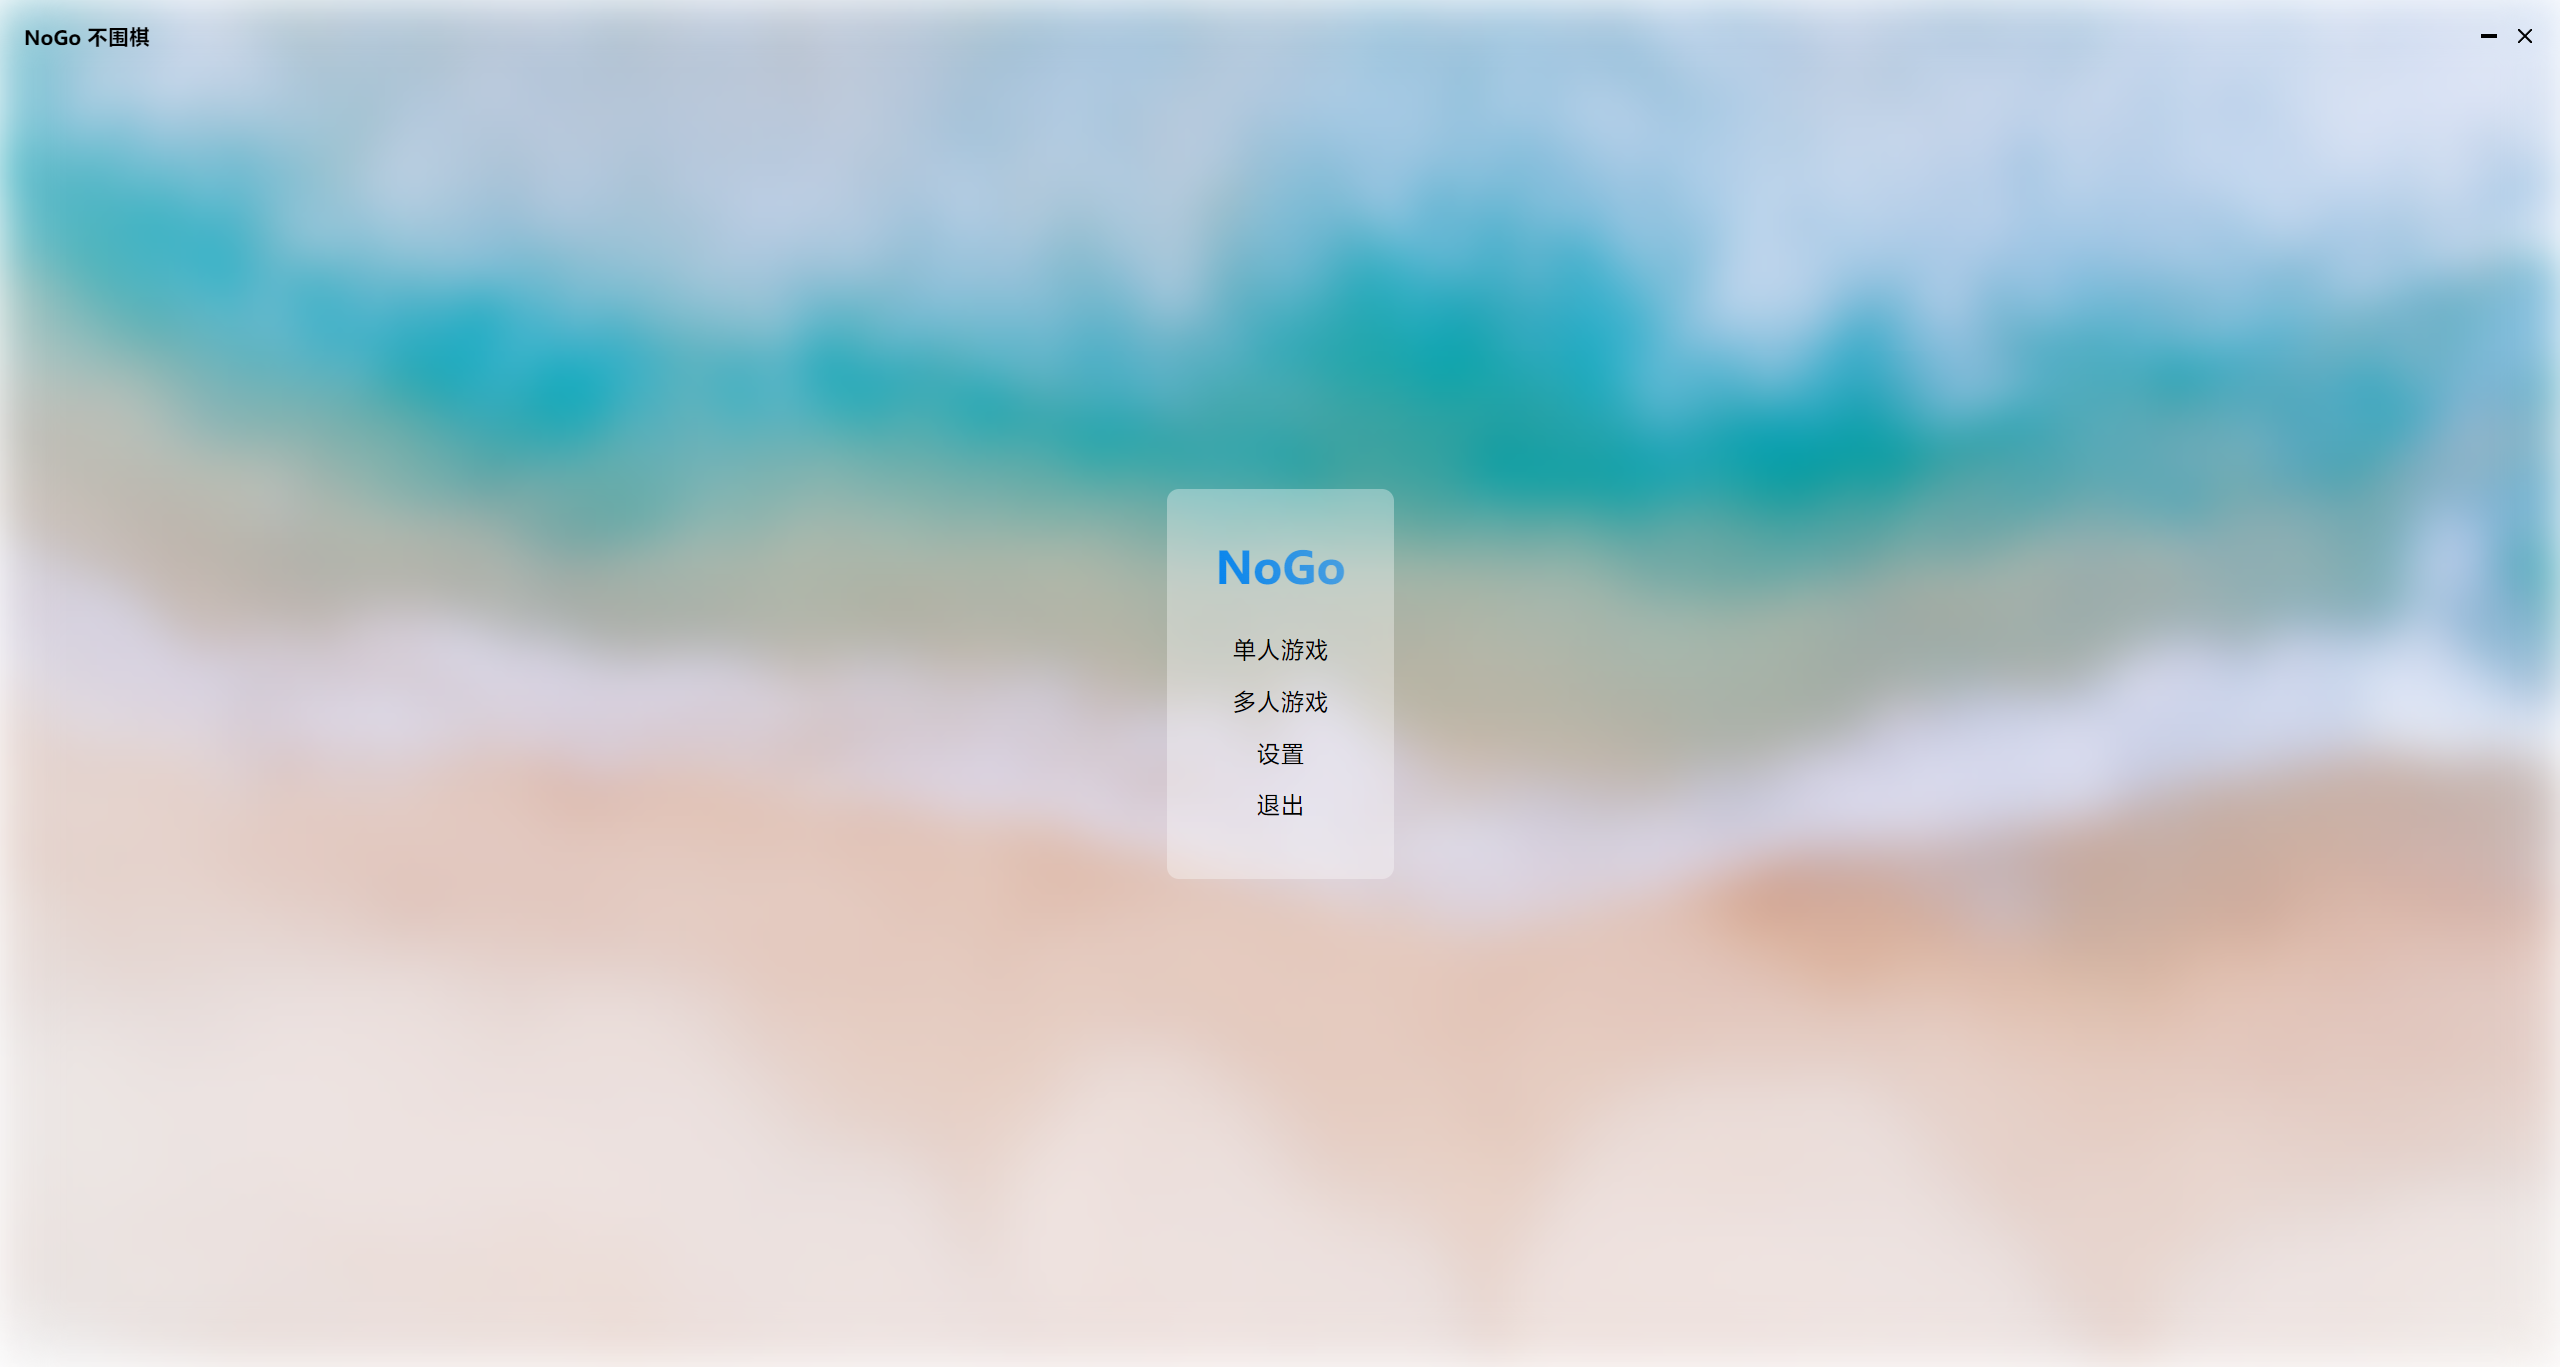
\includegraphics[width=11cm]{Images/Home.png}
	\caption{主页}
\end{figure}
联机界面左侧最上方显示了用户名,可以直接修改;中间是本机的局域网地址,可以方便地告知对方;下面可以输入对方的 IP 地址和端口号来发起对局申请。右侧是一个列表\footnote{实际上,当前版本只会显示一个请求(即队列中的第一个请求)},显示当前已经收到的对局请求。\par
\begin{figure}[H]
	\centering
	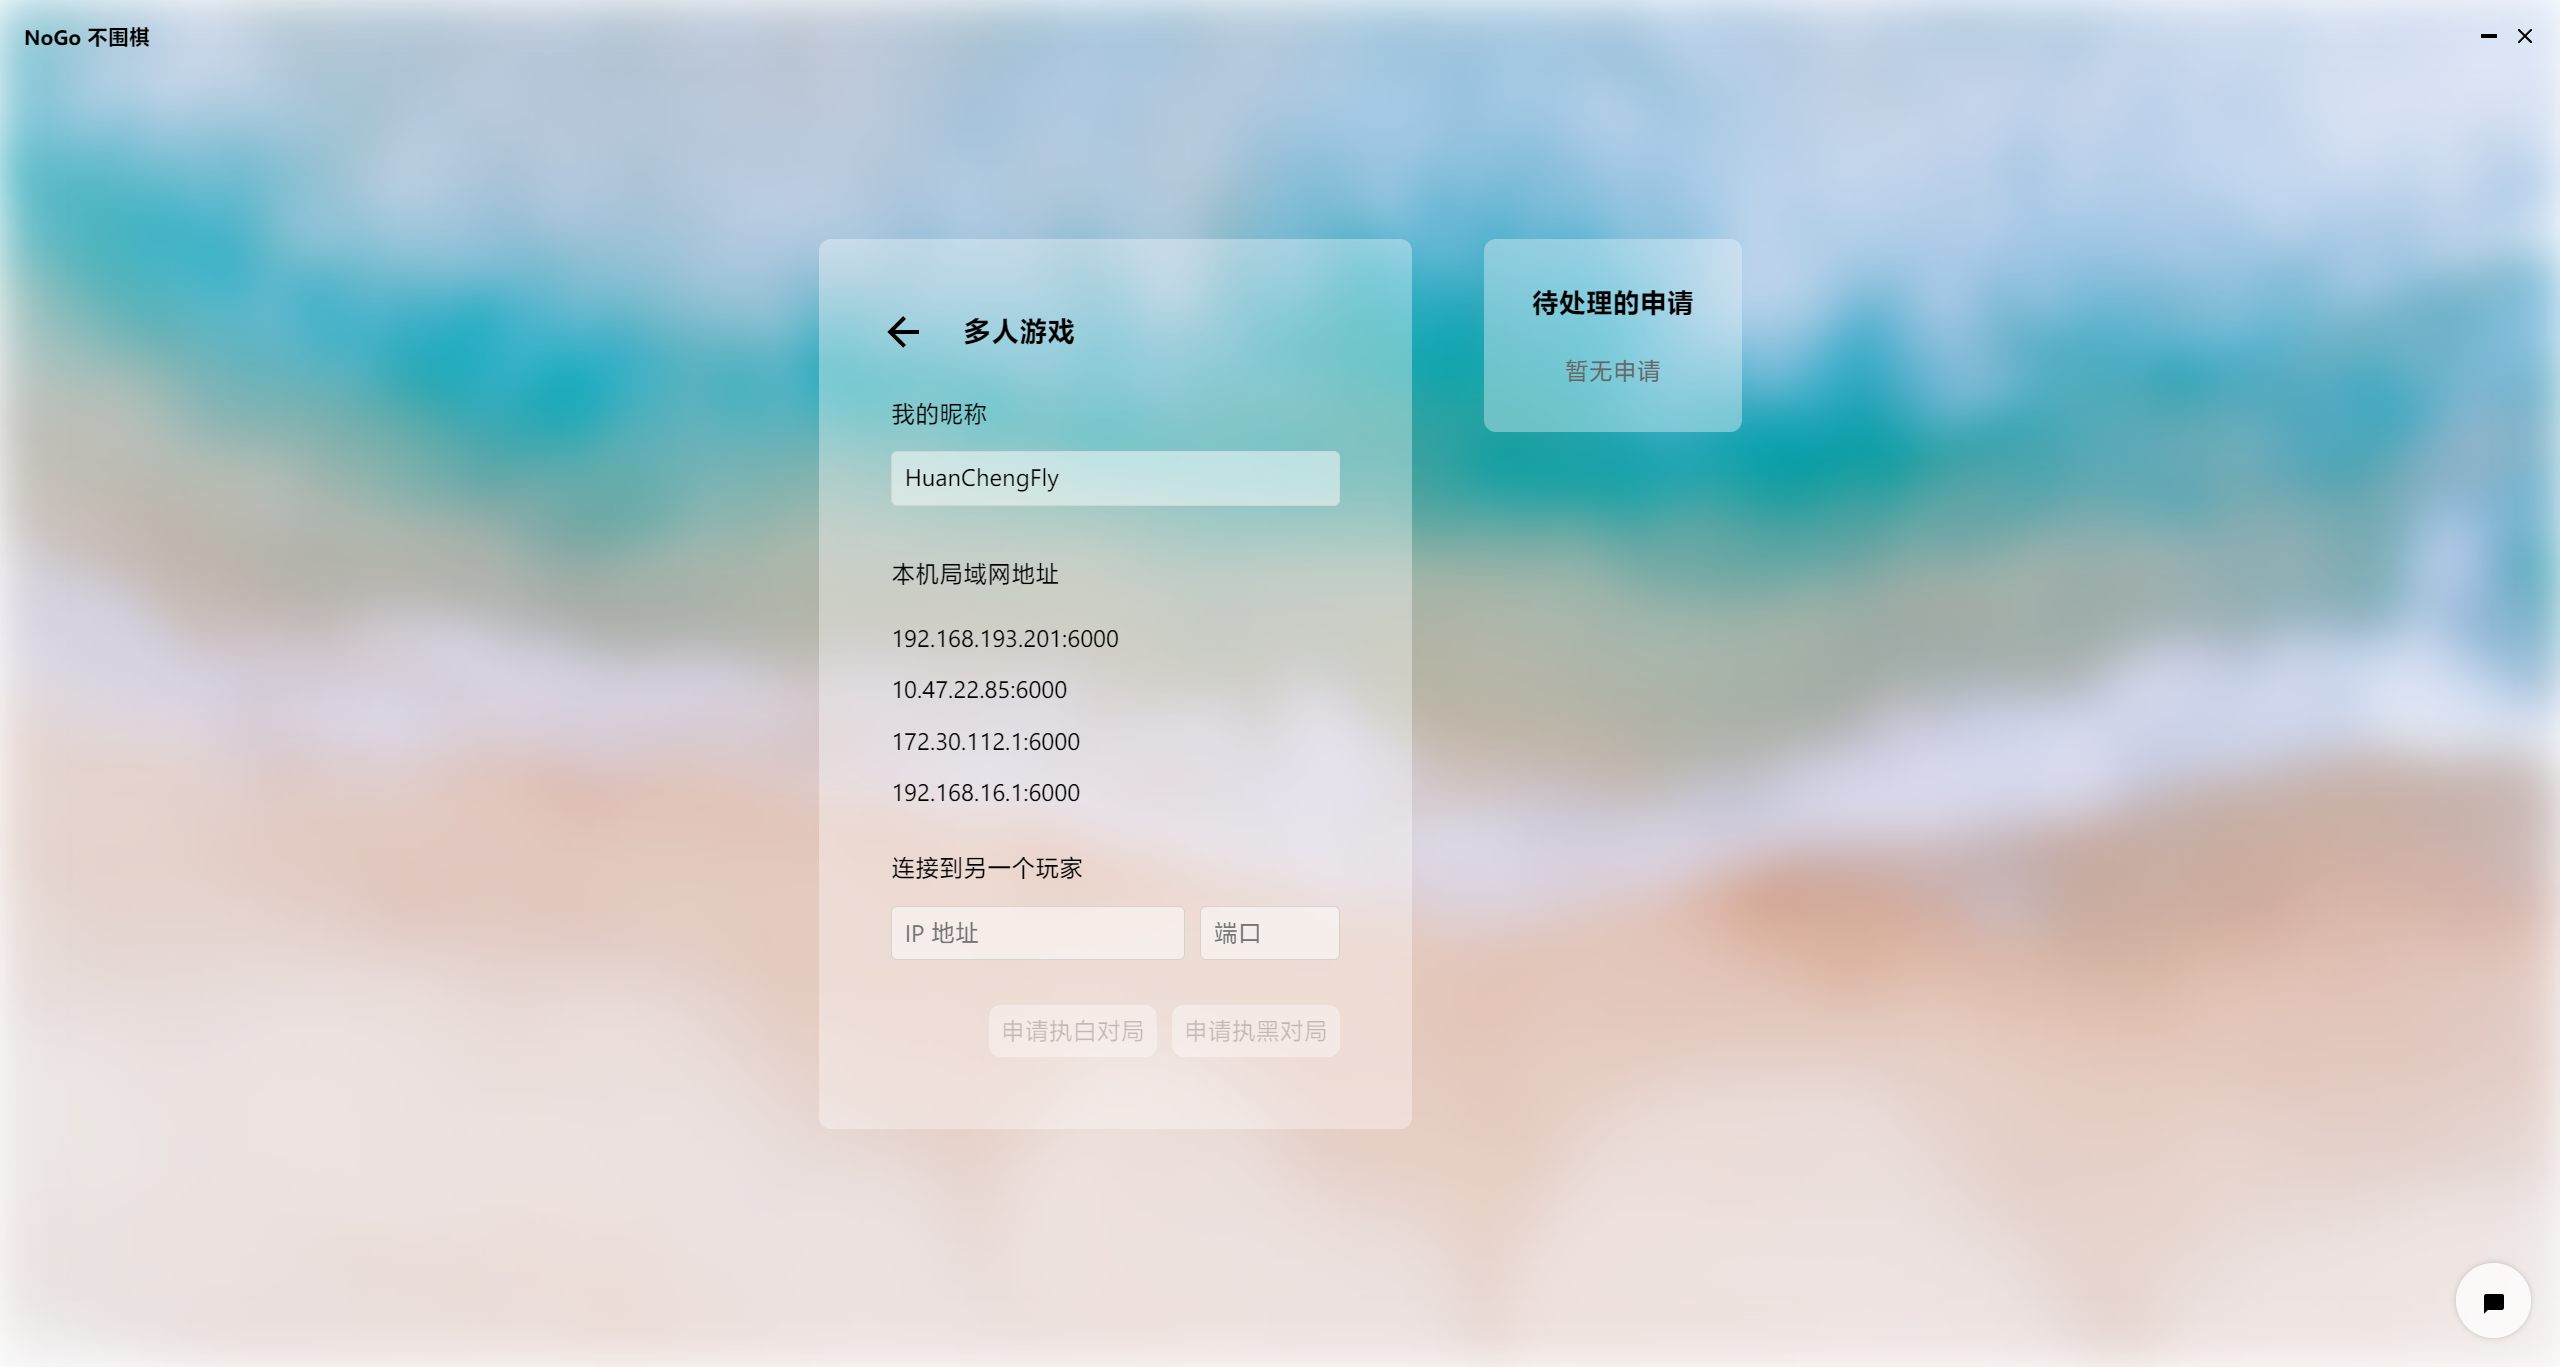
\includegraphics[width=11cm]{Images/OnlinePlay.png}
	\caption{联机游戏界面}
\end{figure}
\begin{figure}[H]
	\begin{minipage}[t]{0.48\textwidth}
		\centering
		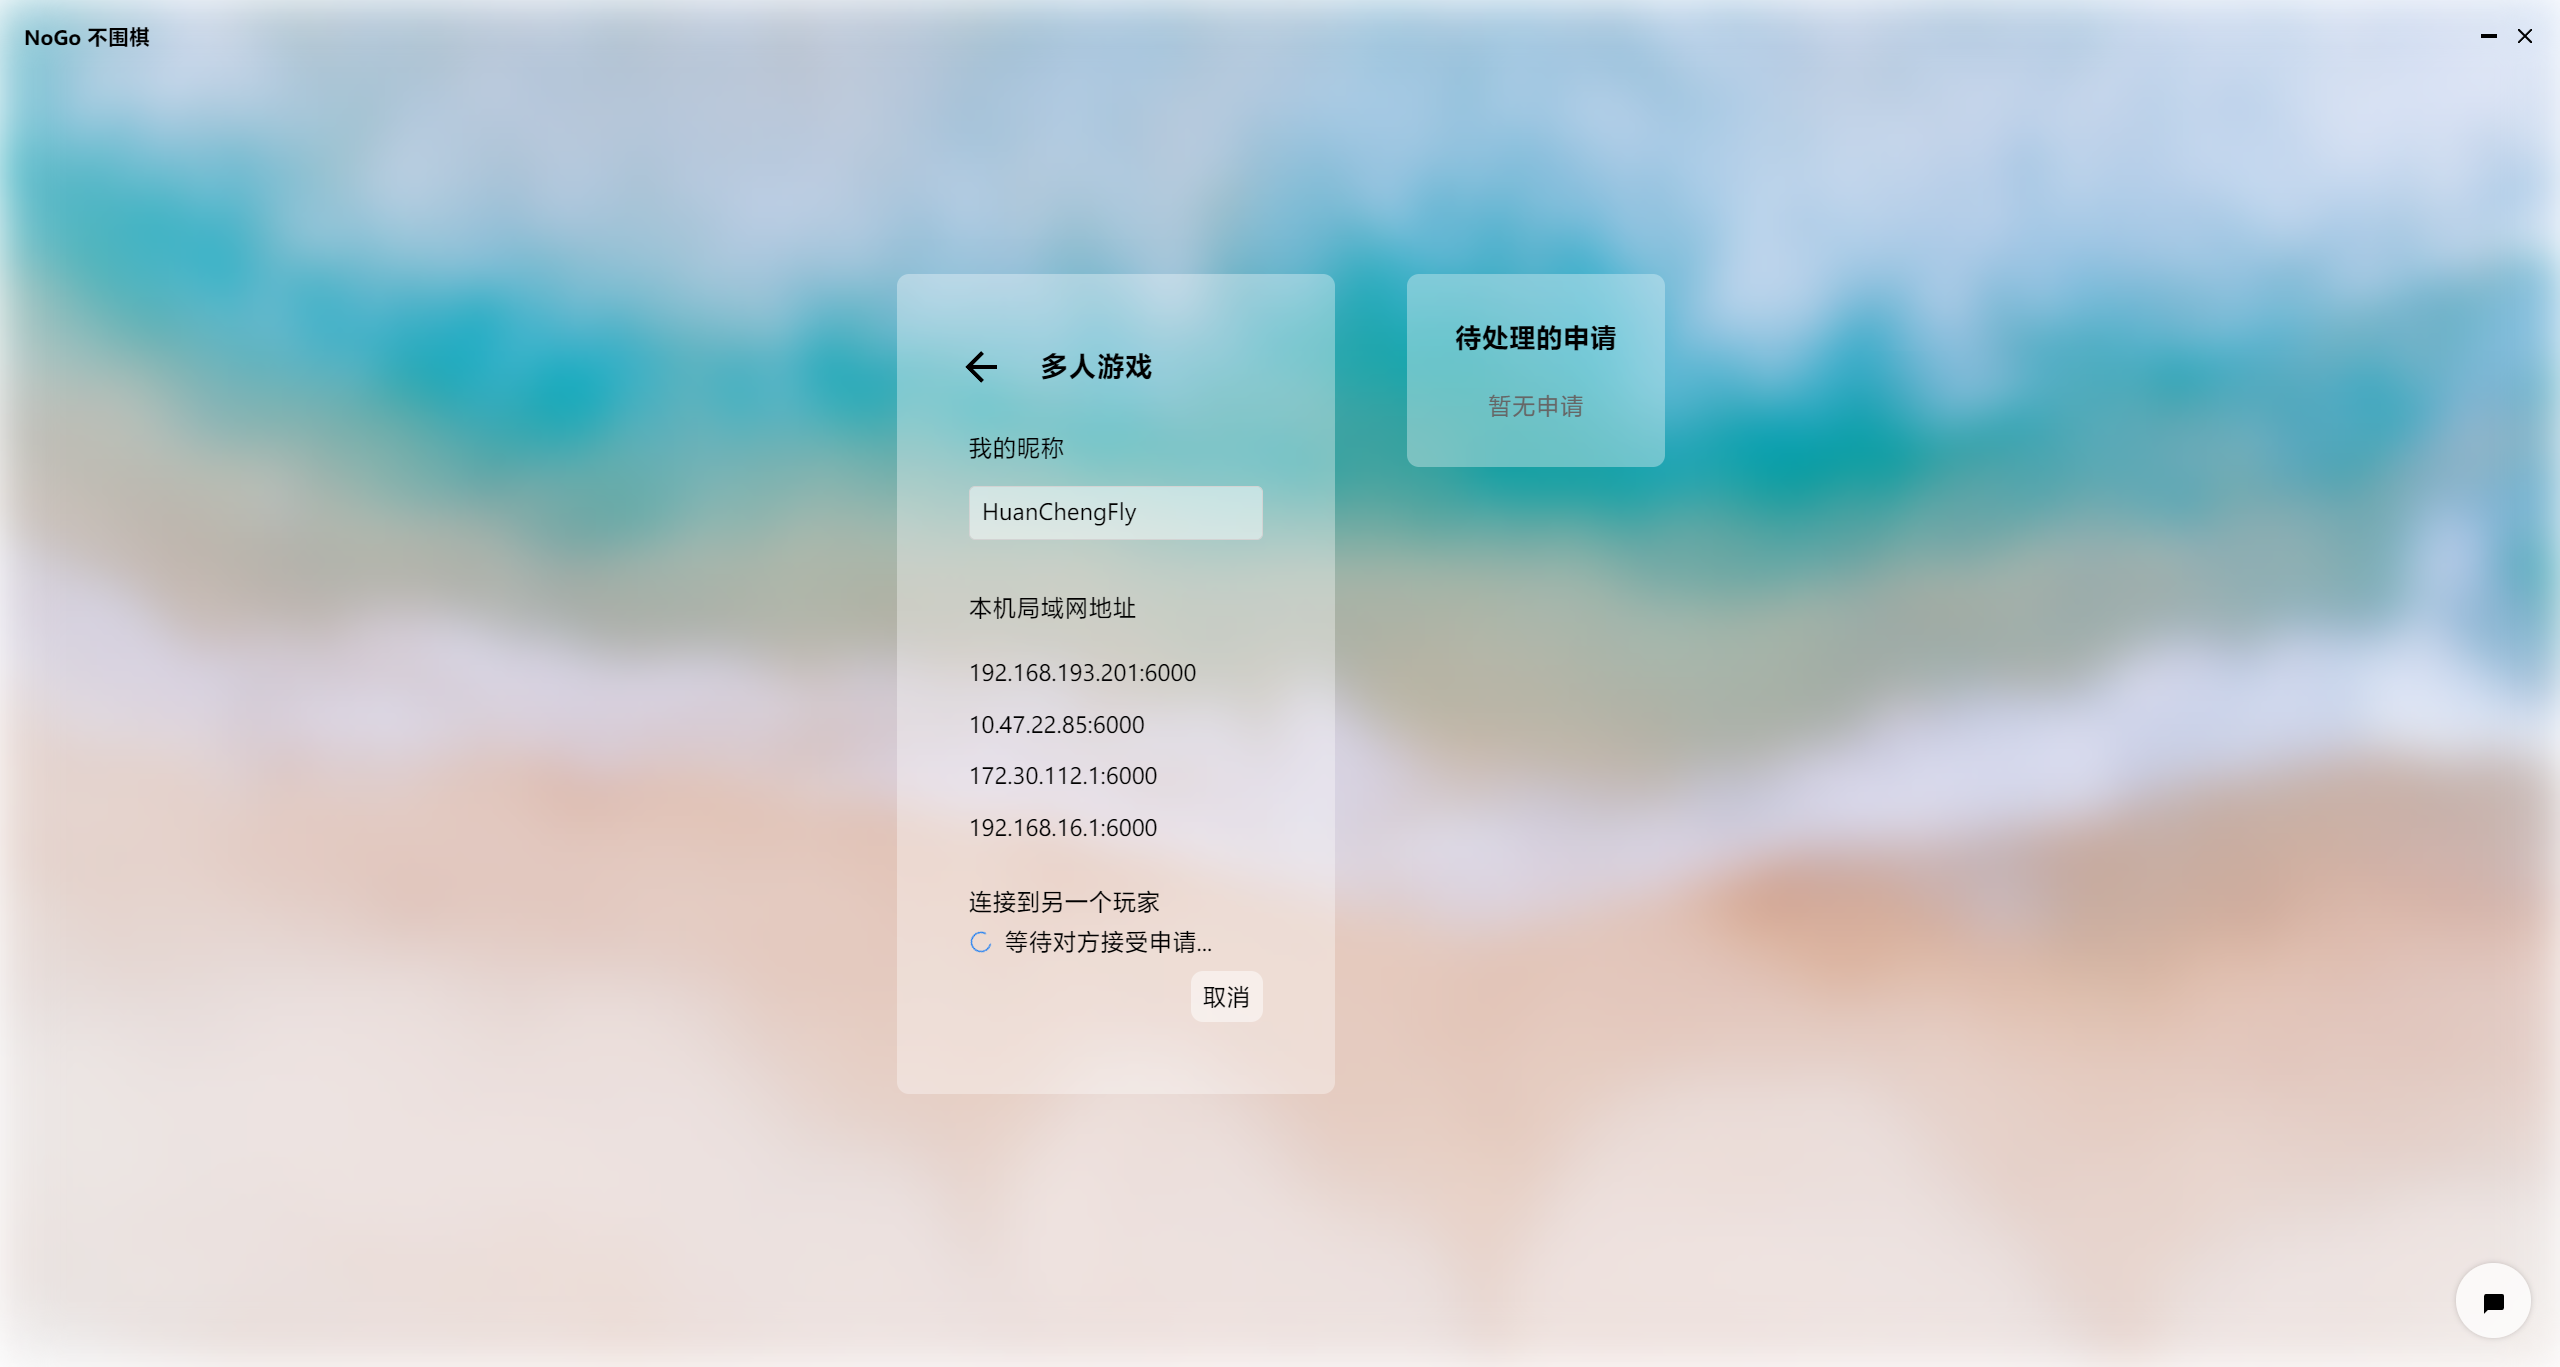
\includegraphics[width=7cm]{Images/Waiting.png}
		\caption{发送对局申请}
	\end{minipage}
	\begin{minipage}[t]{0.48\textwidth}
		\centering
		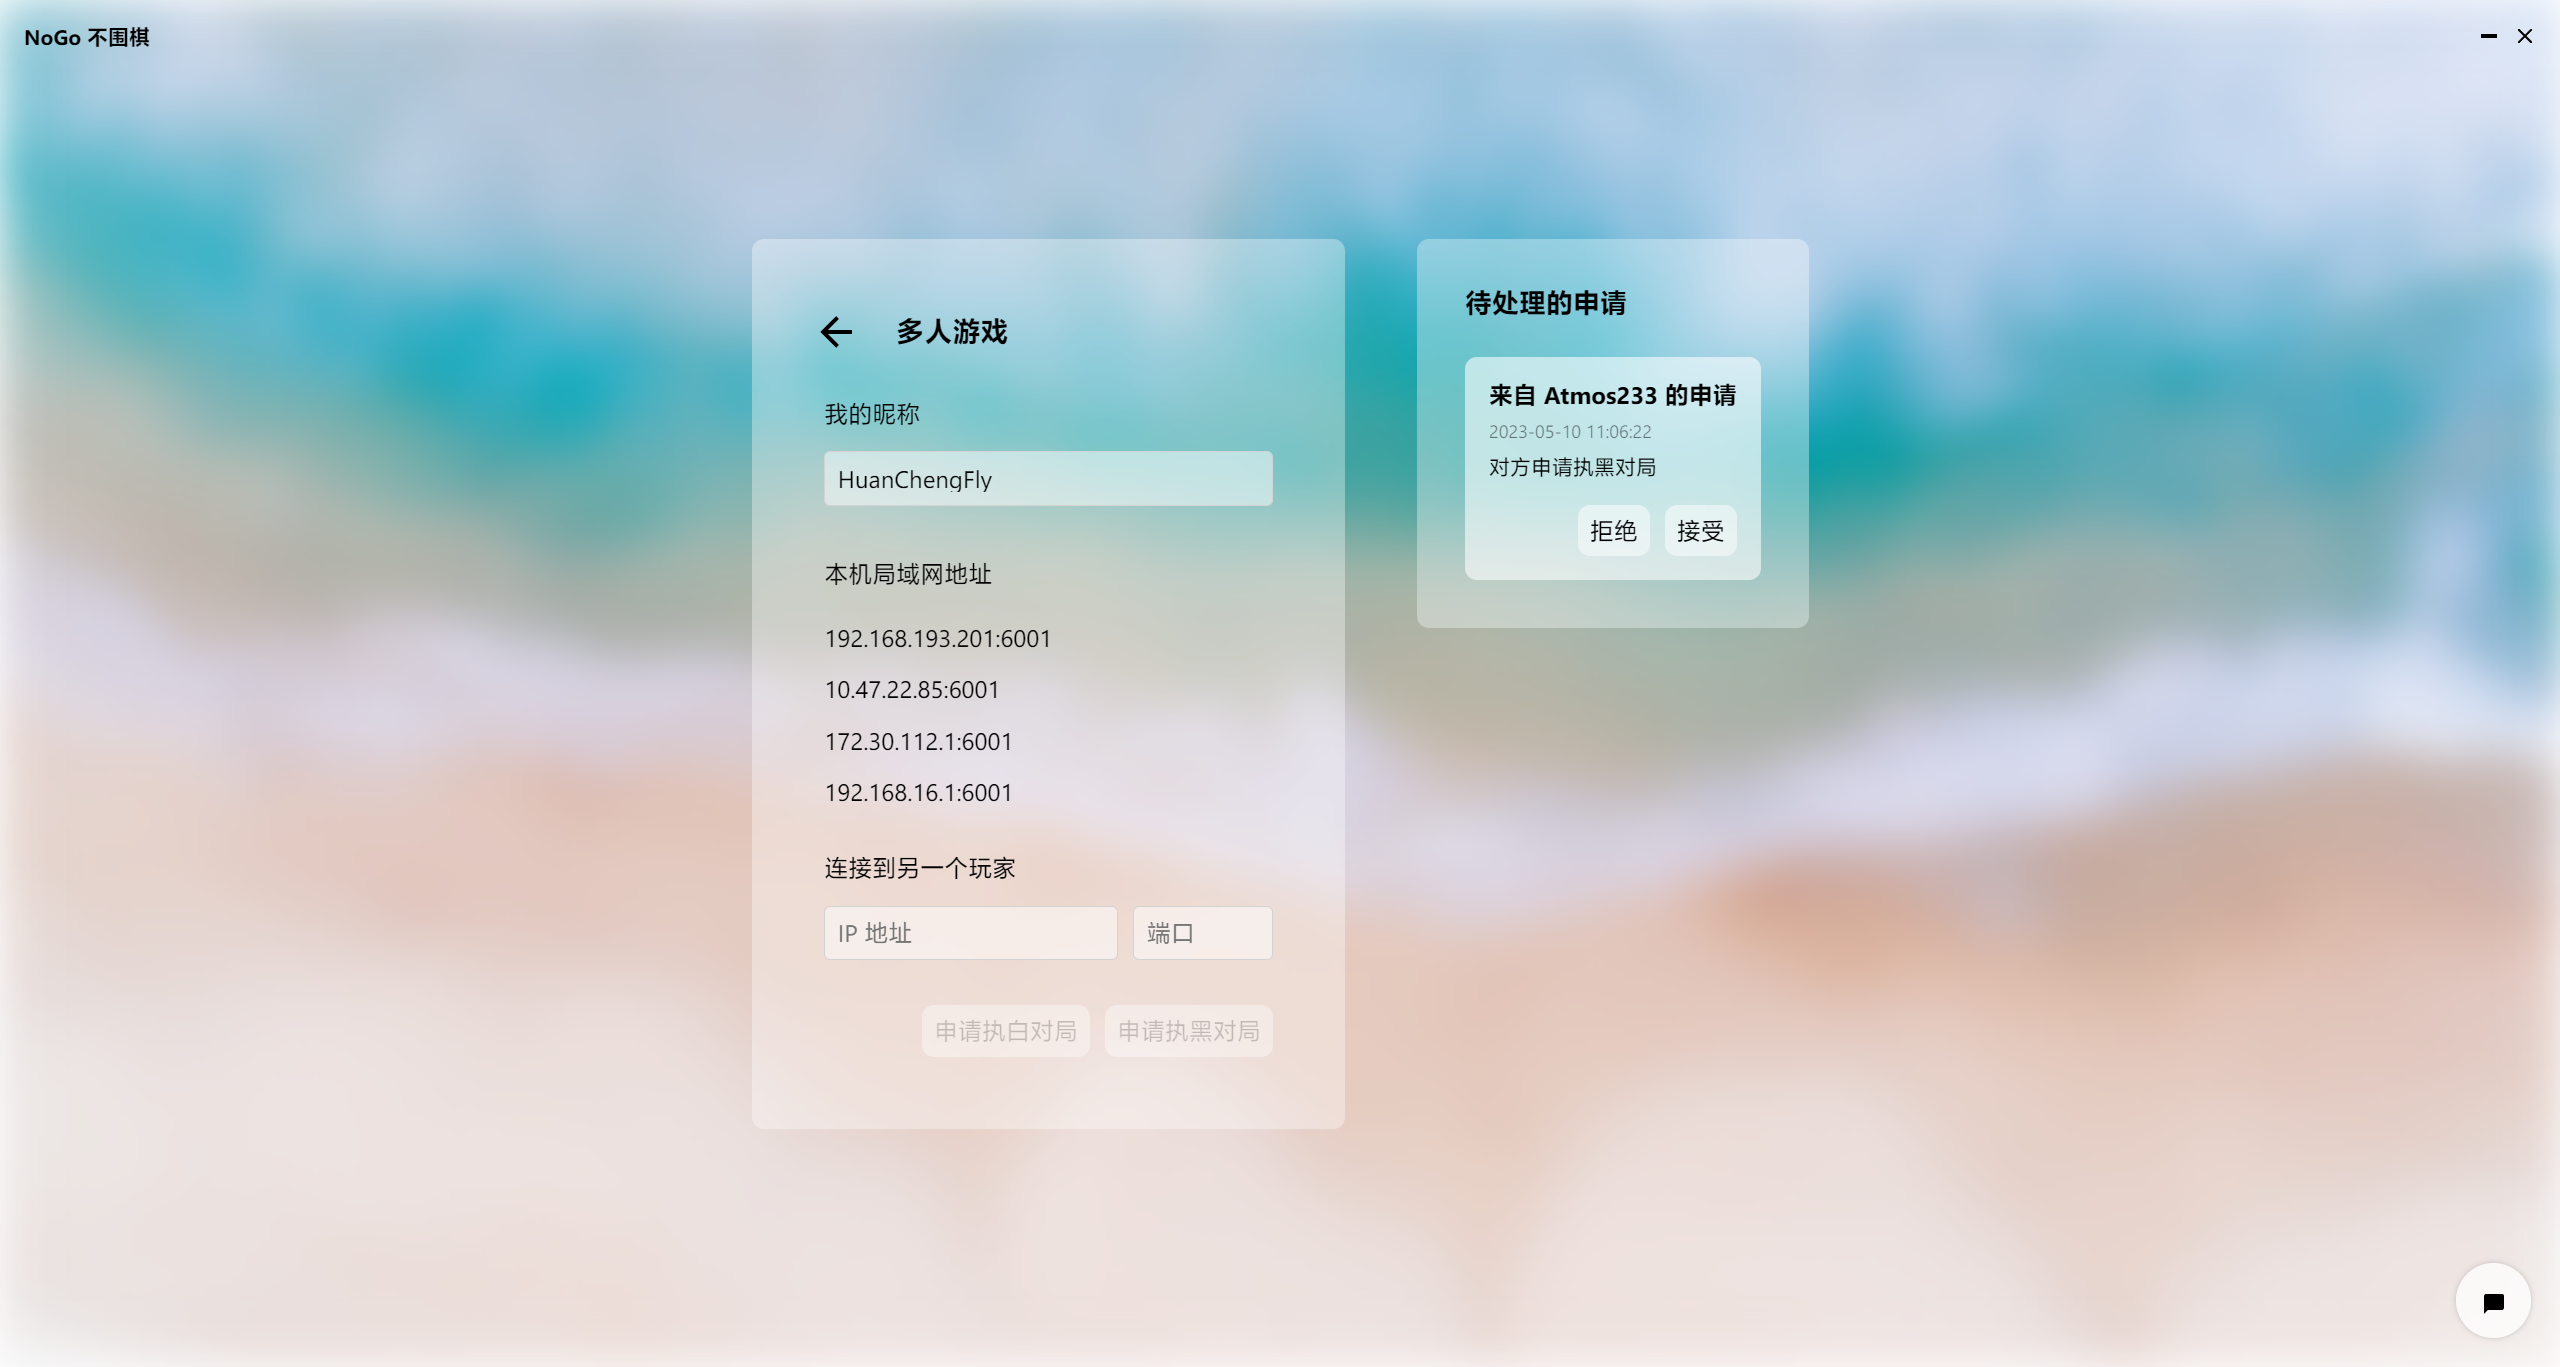
\includegraphics[width=7cm]{Images/ReceiveRequest.png}
		\caption{收到对局申请}
	\end{minipage}
\end{figure}
若申请被拒绝,用户可以选择重新发送申请、与对方进行聊天或者直接断开连接。\par
\begin{figure}[H]
	\begin{minipage}[t]{0.48\textwidth}
		\centering
		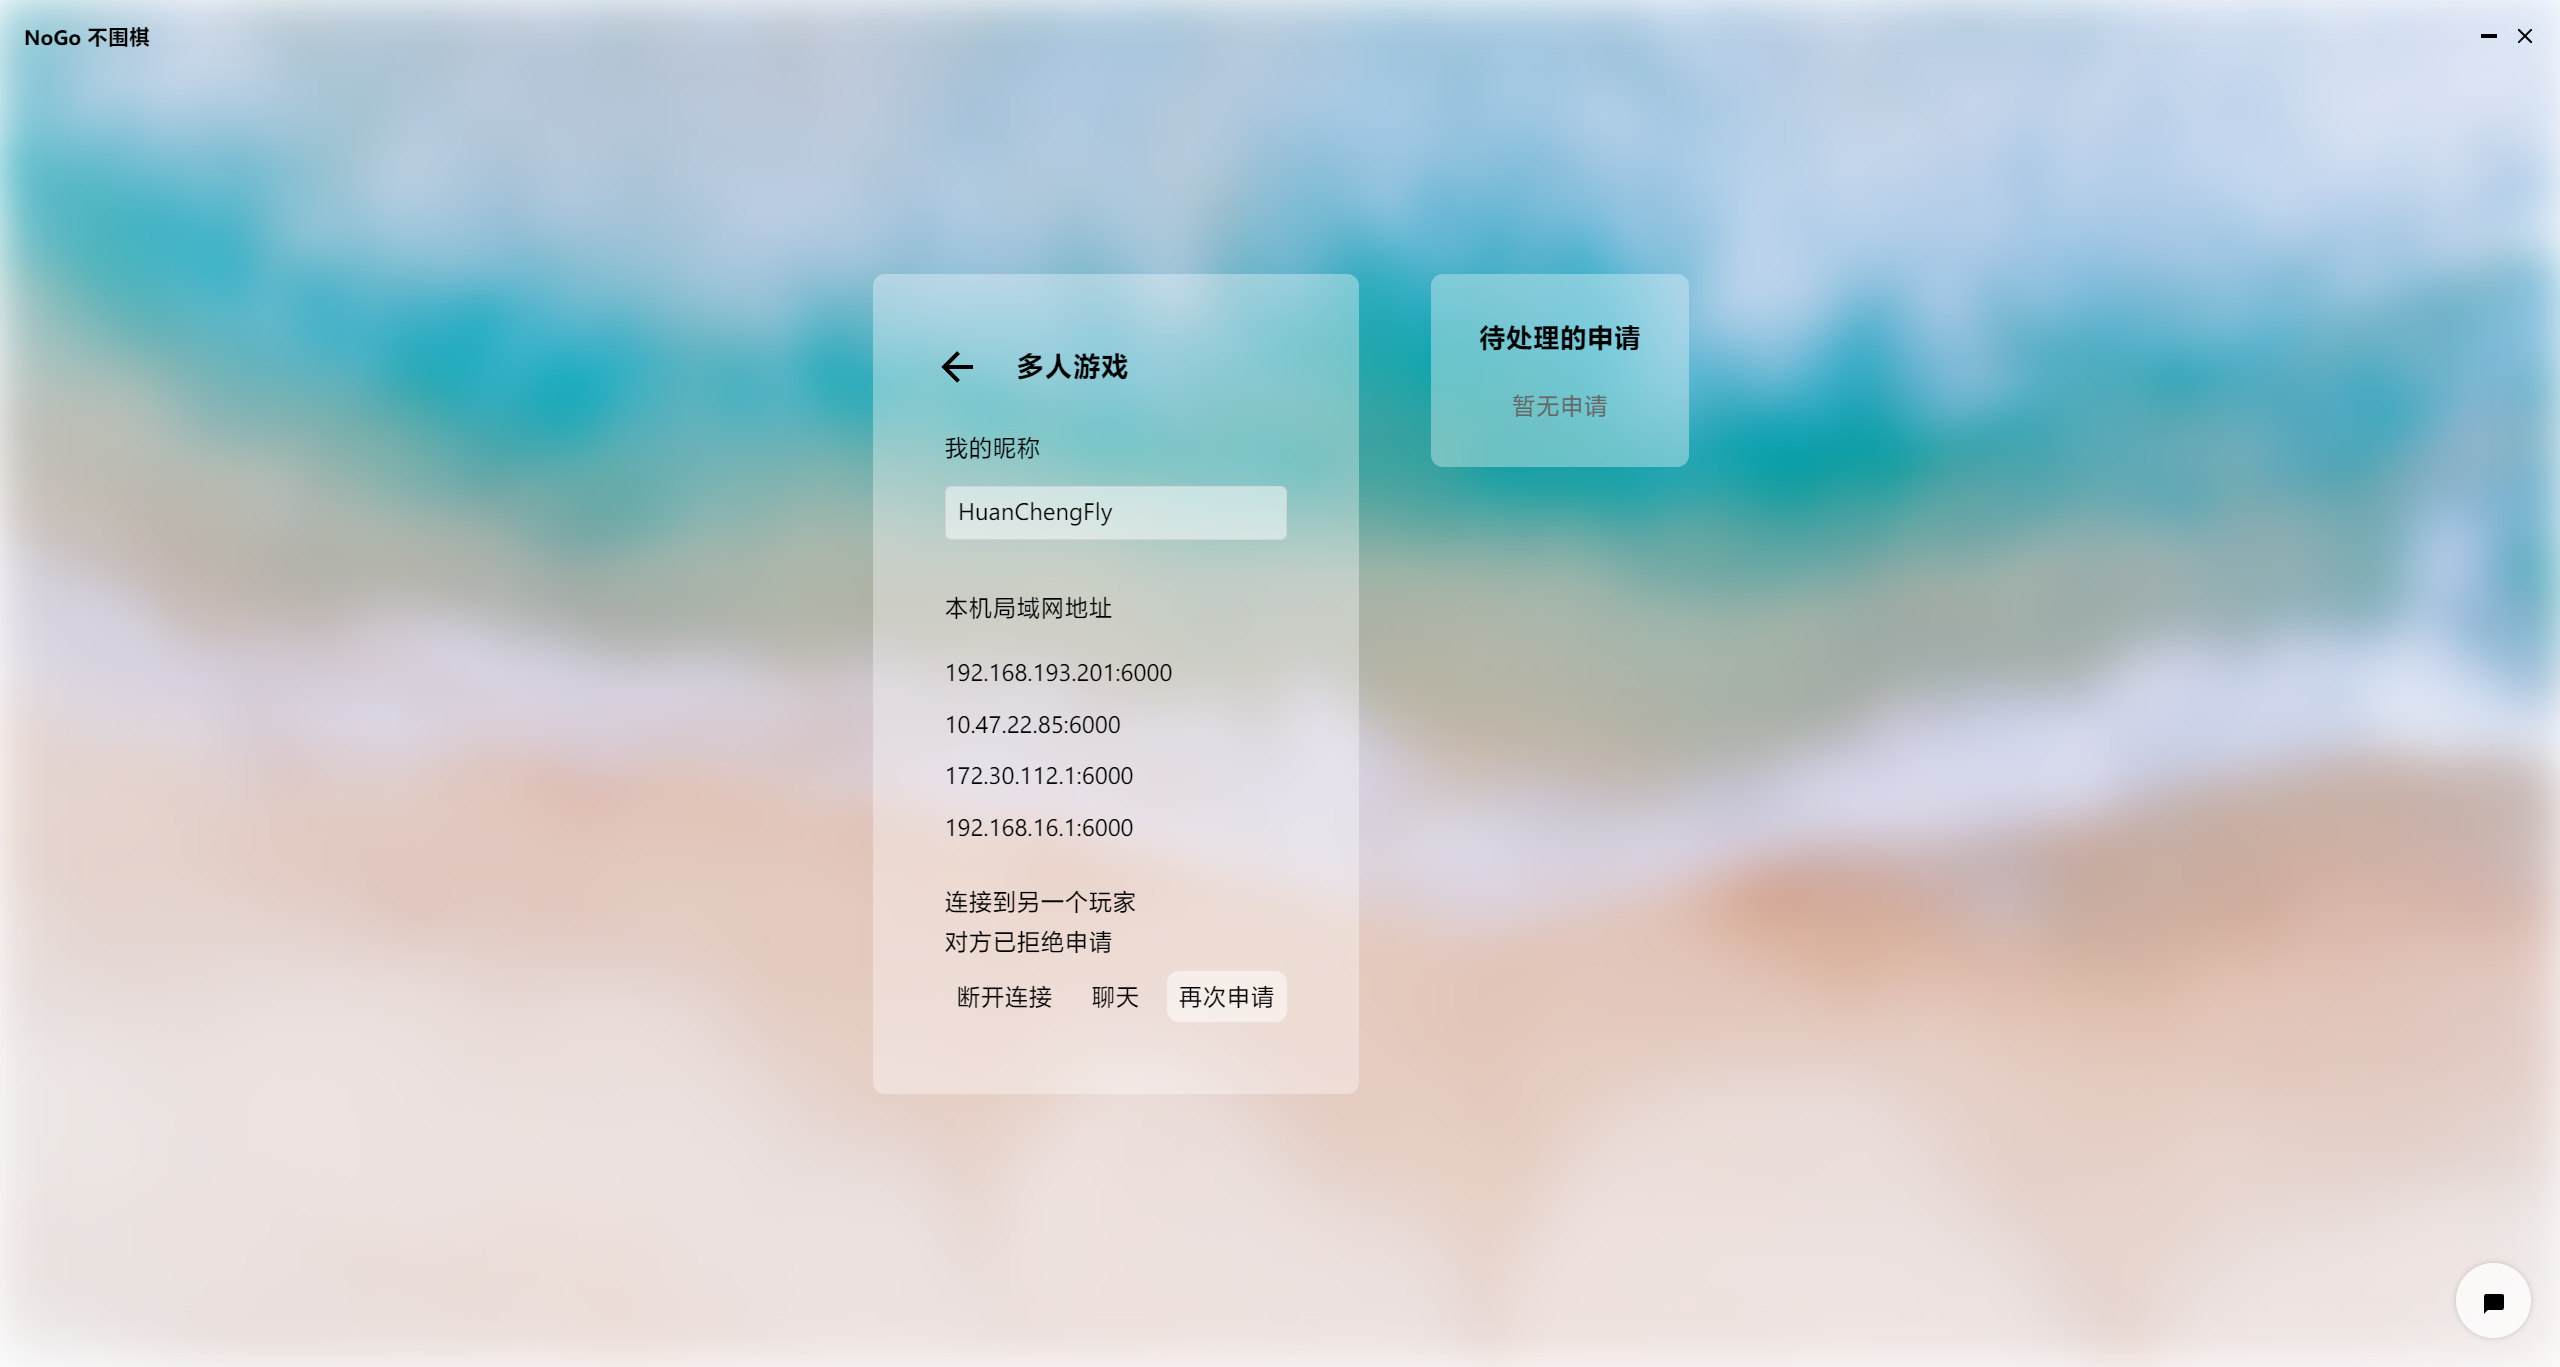
\includegraphics[width=7cm]{Images/Rejected.png}
		\caption{对局申请被拒绝}
	\end{minipage}
	\begin{minipage}[t]{0.48\textwidth}
		\centering
		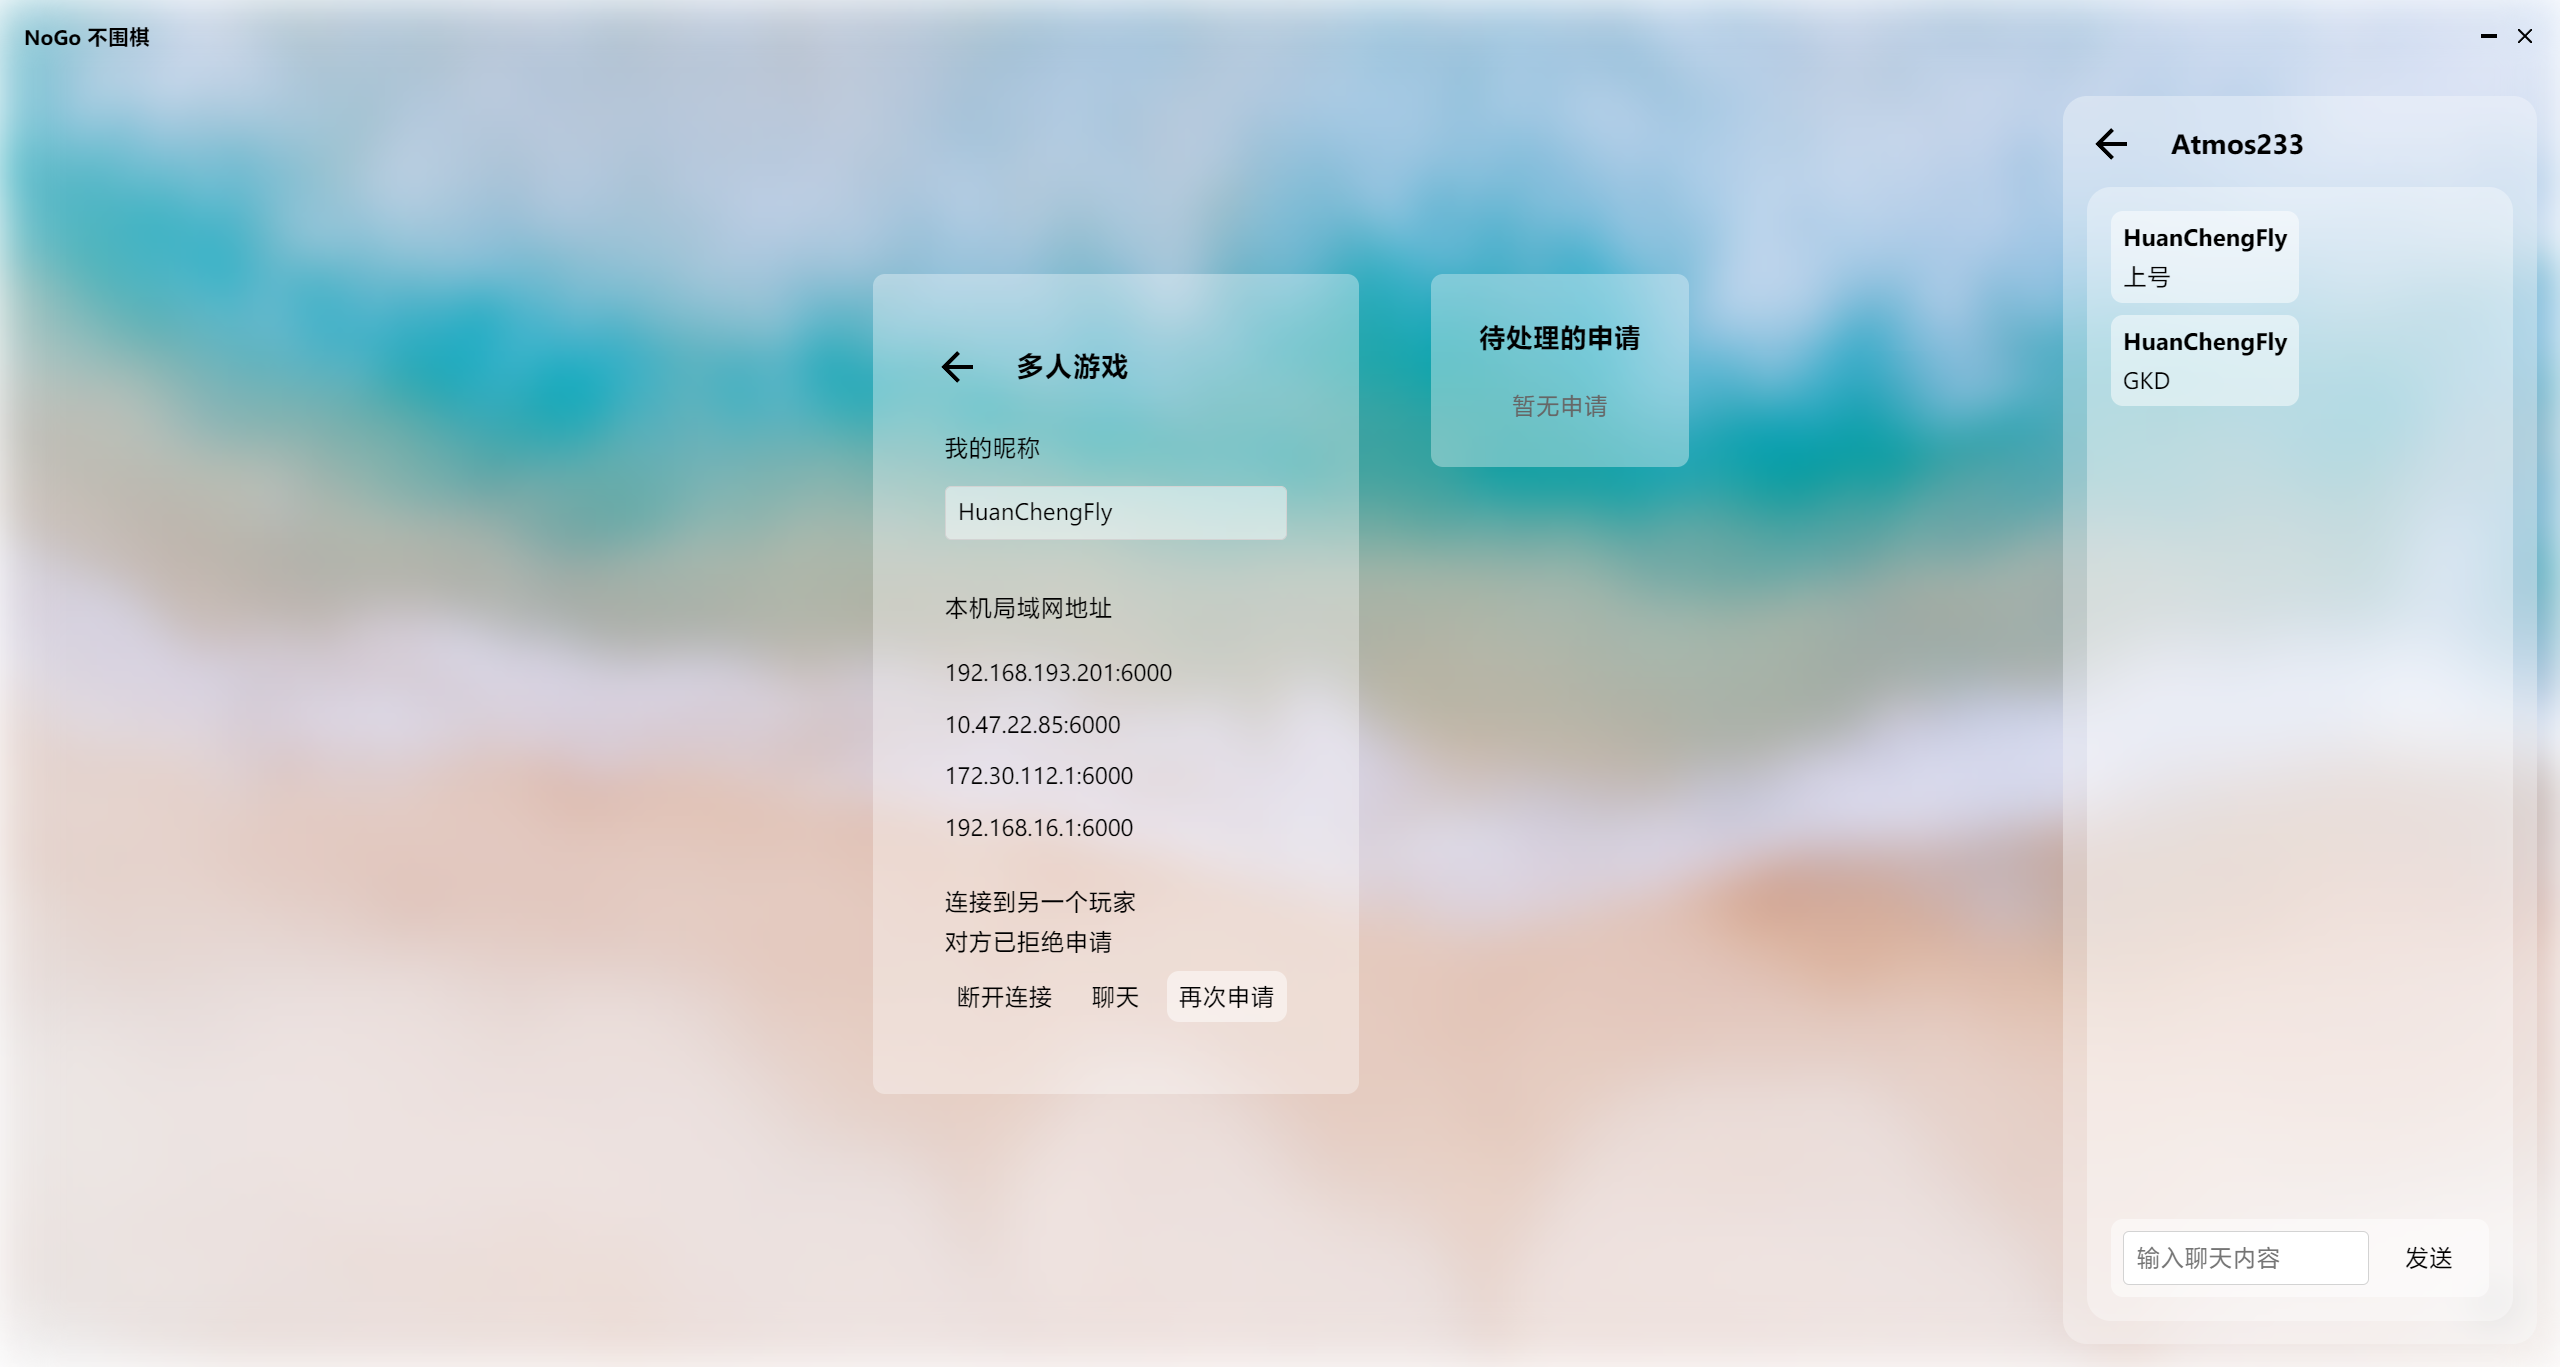
\includegraphics[width=7cm]{Images/ChatWhenRejected.png}
		\caption{拒绝时可以发起聊天}
	\end{minipage}
\end{figure}
此外,由于我们在启动时就开始监听联机端口,因此即使不在联机游戏界面依然能收到对局申请,以弹窗的形式显示在界面右上角。\par
\begin{figure}[H]
	\centering
	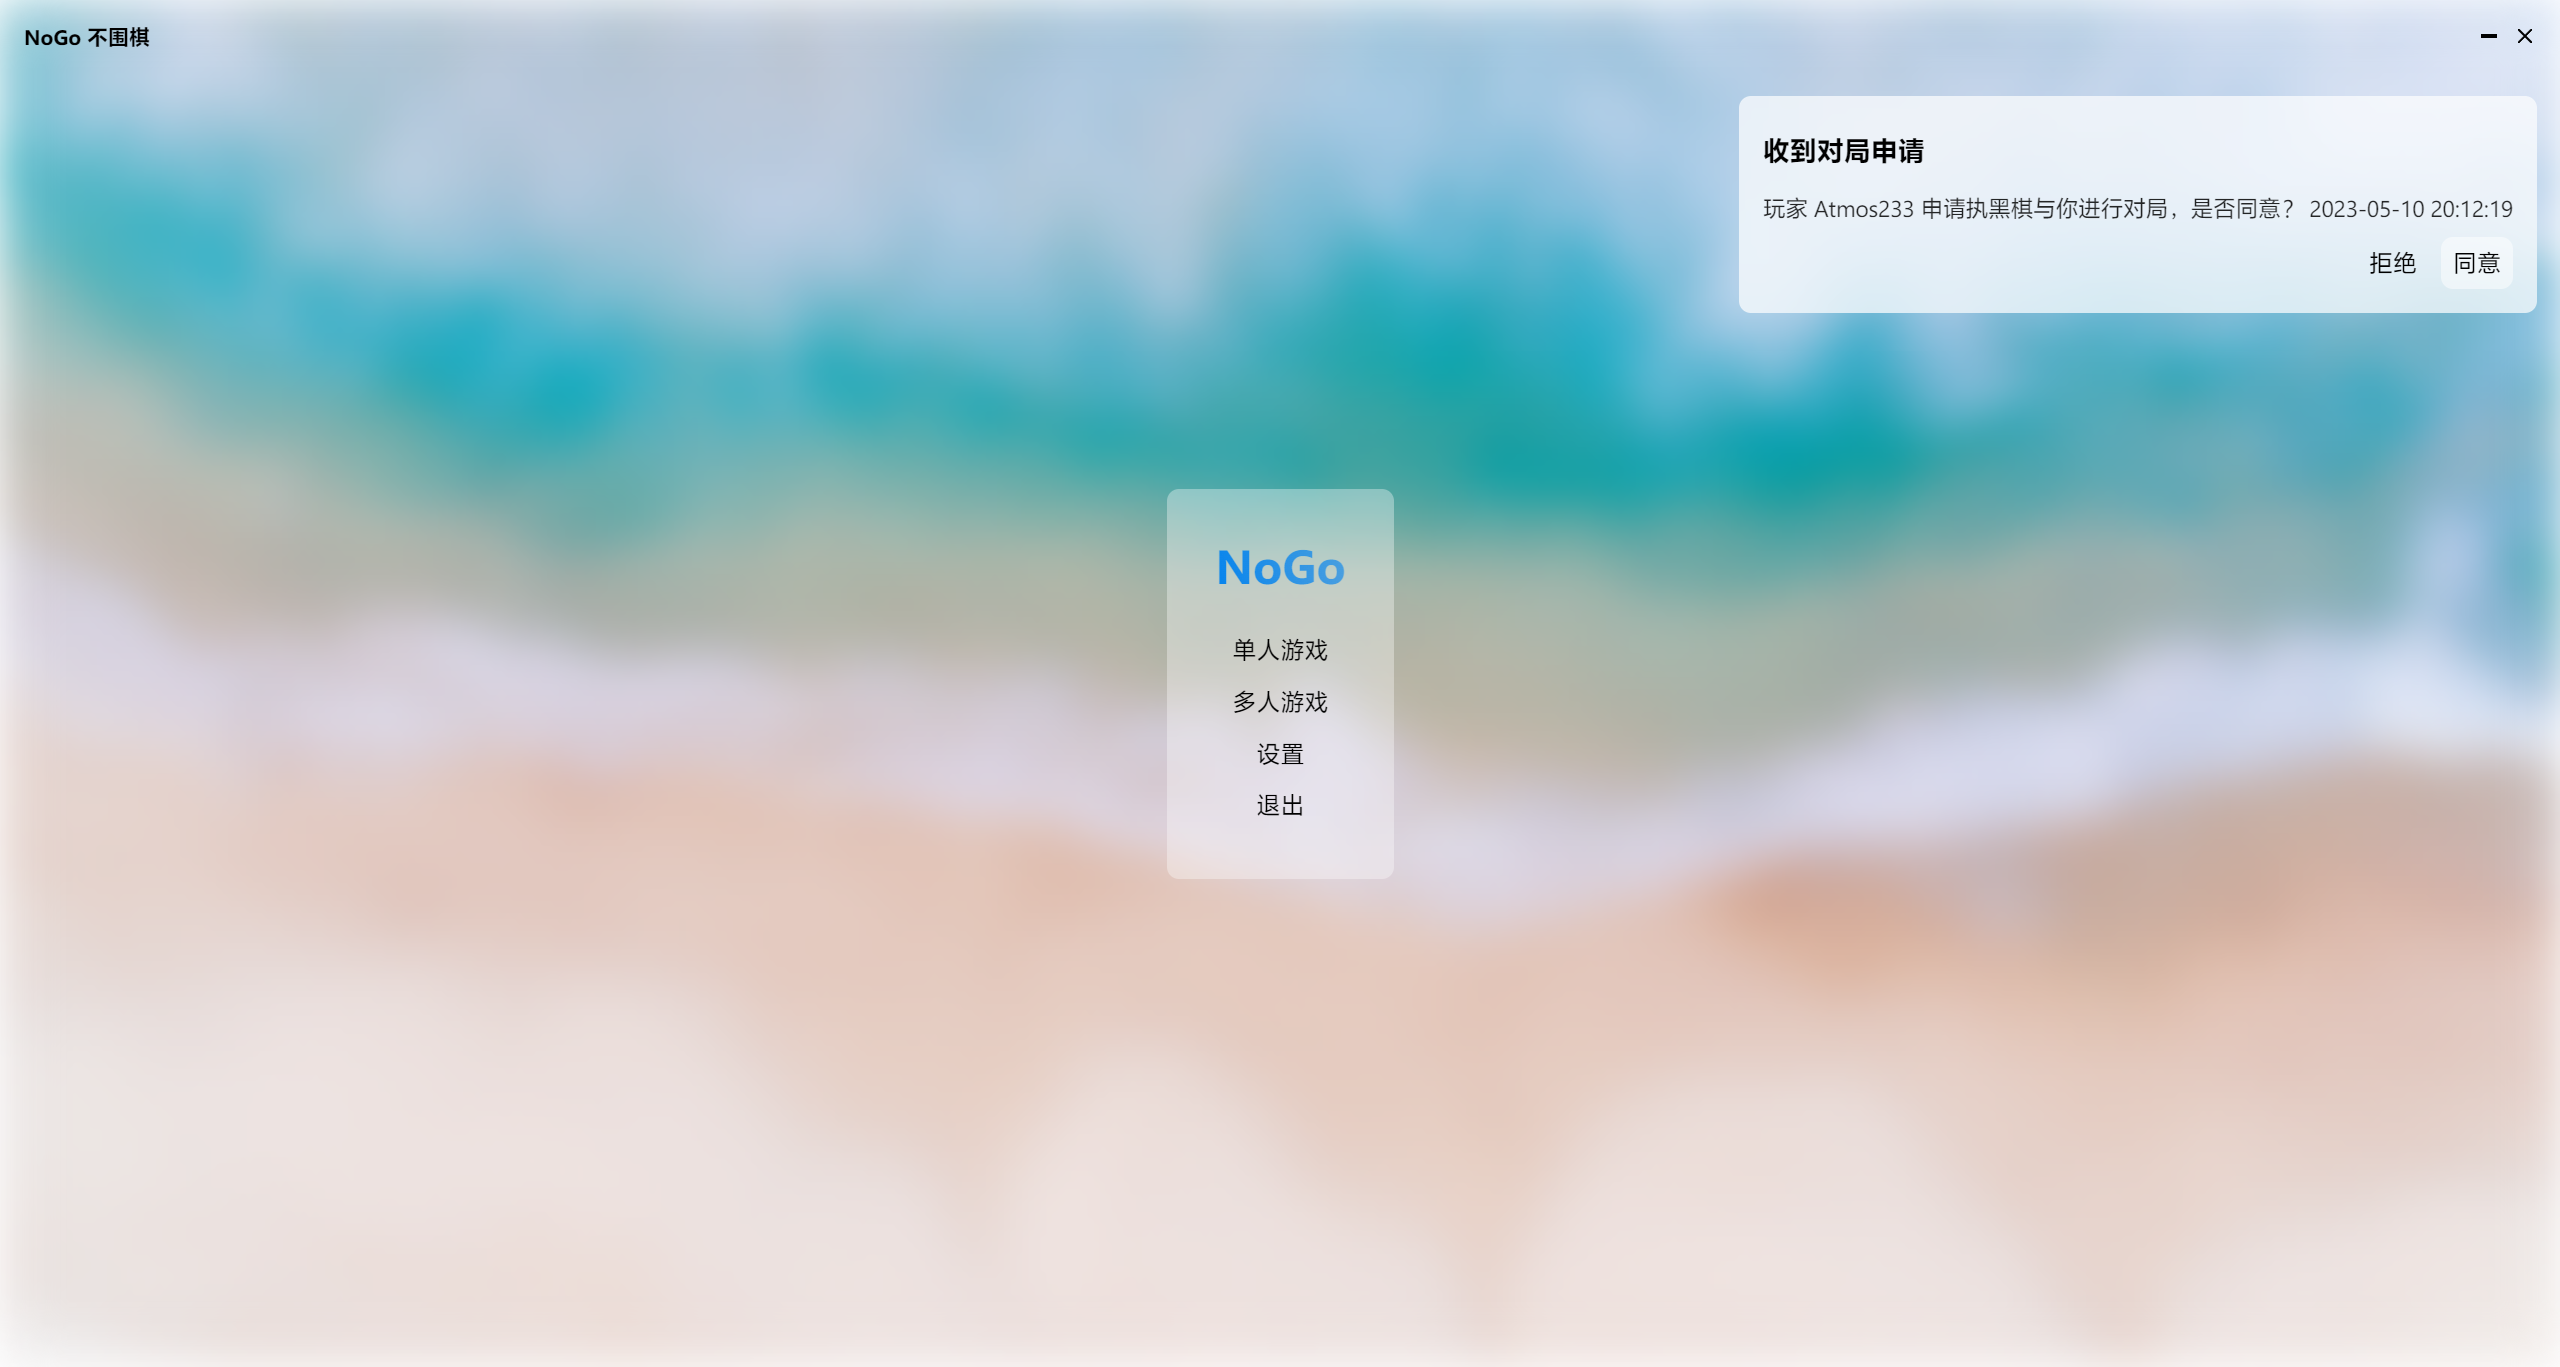
\includegraphics[width=11cm]{Images/ReceiveResultAtHome.png}
	\caption{弹窗显示对局申请}
\end{figure}
若申请被接受,游戏即开始,自动跳转至联机对局页面。\par
联机对局页面的左侧是当前棋局的棋盘和对局双方信息;右侧依次是对局信息(当前包括用时、步数),认输按钮和聊天窗口。\par
这一版本中我们将计时器的显示方法更改为了“剩余时间”而非之前的“已用时间”。\par
\begin{figure}[H]
	\centering
	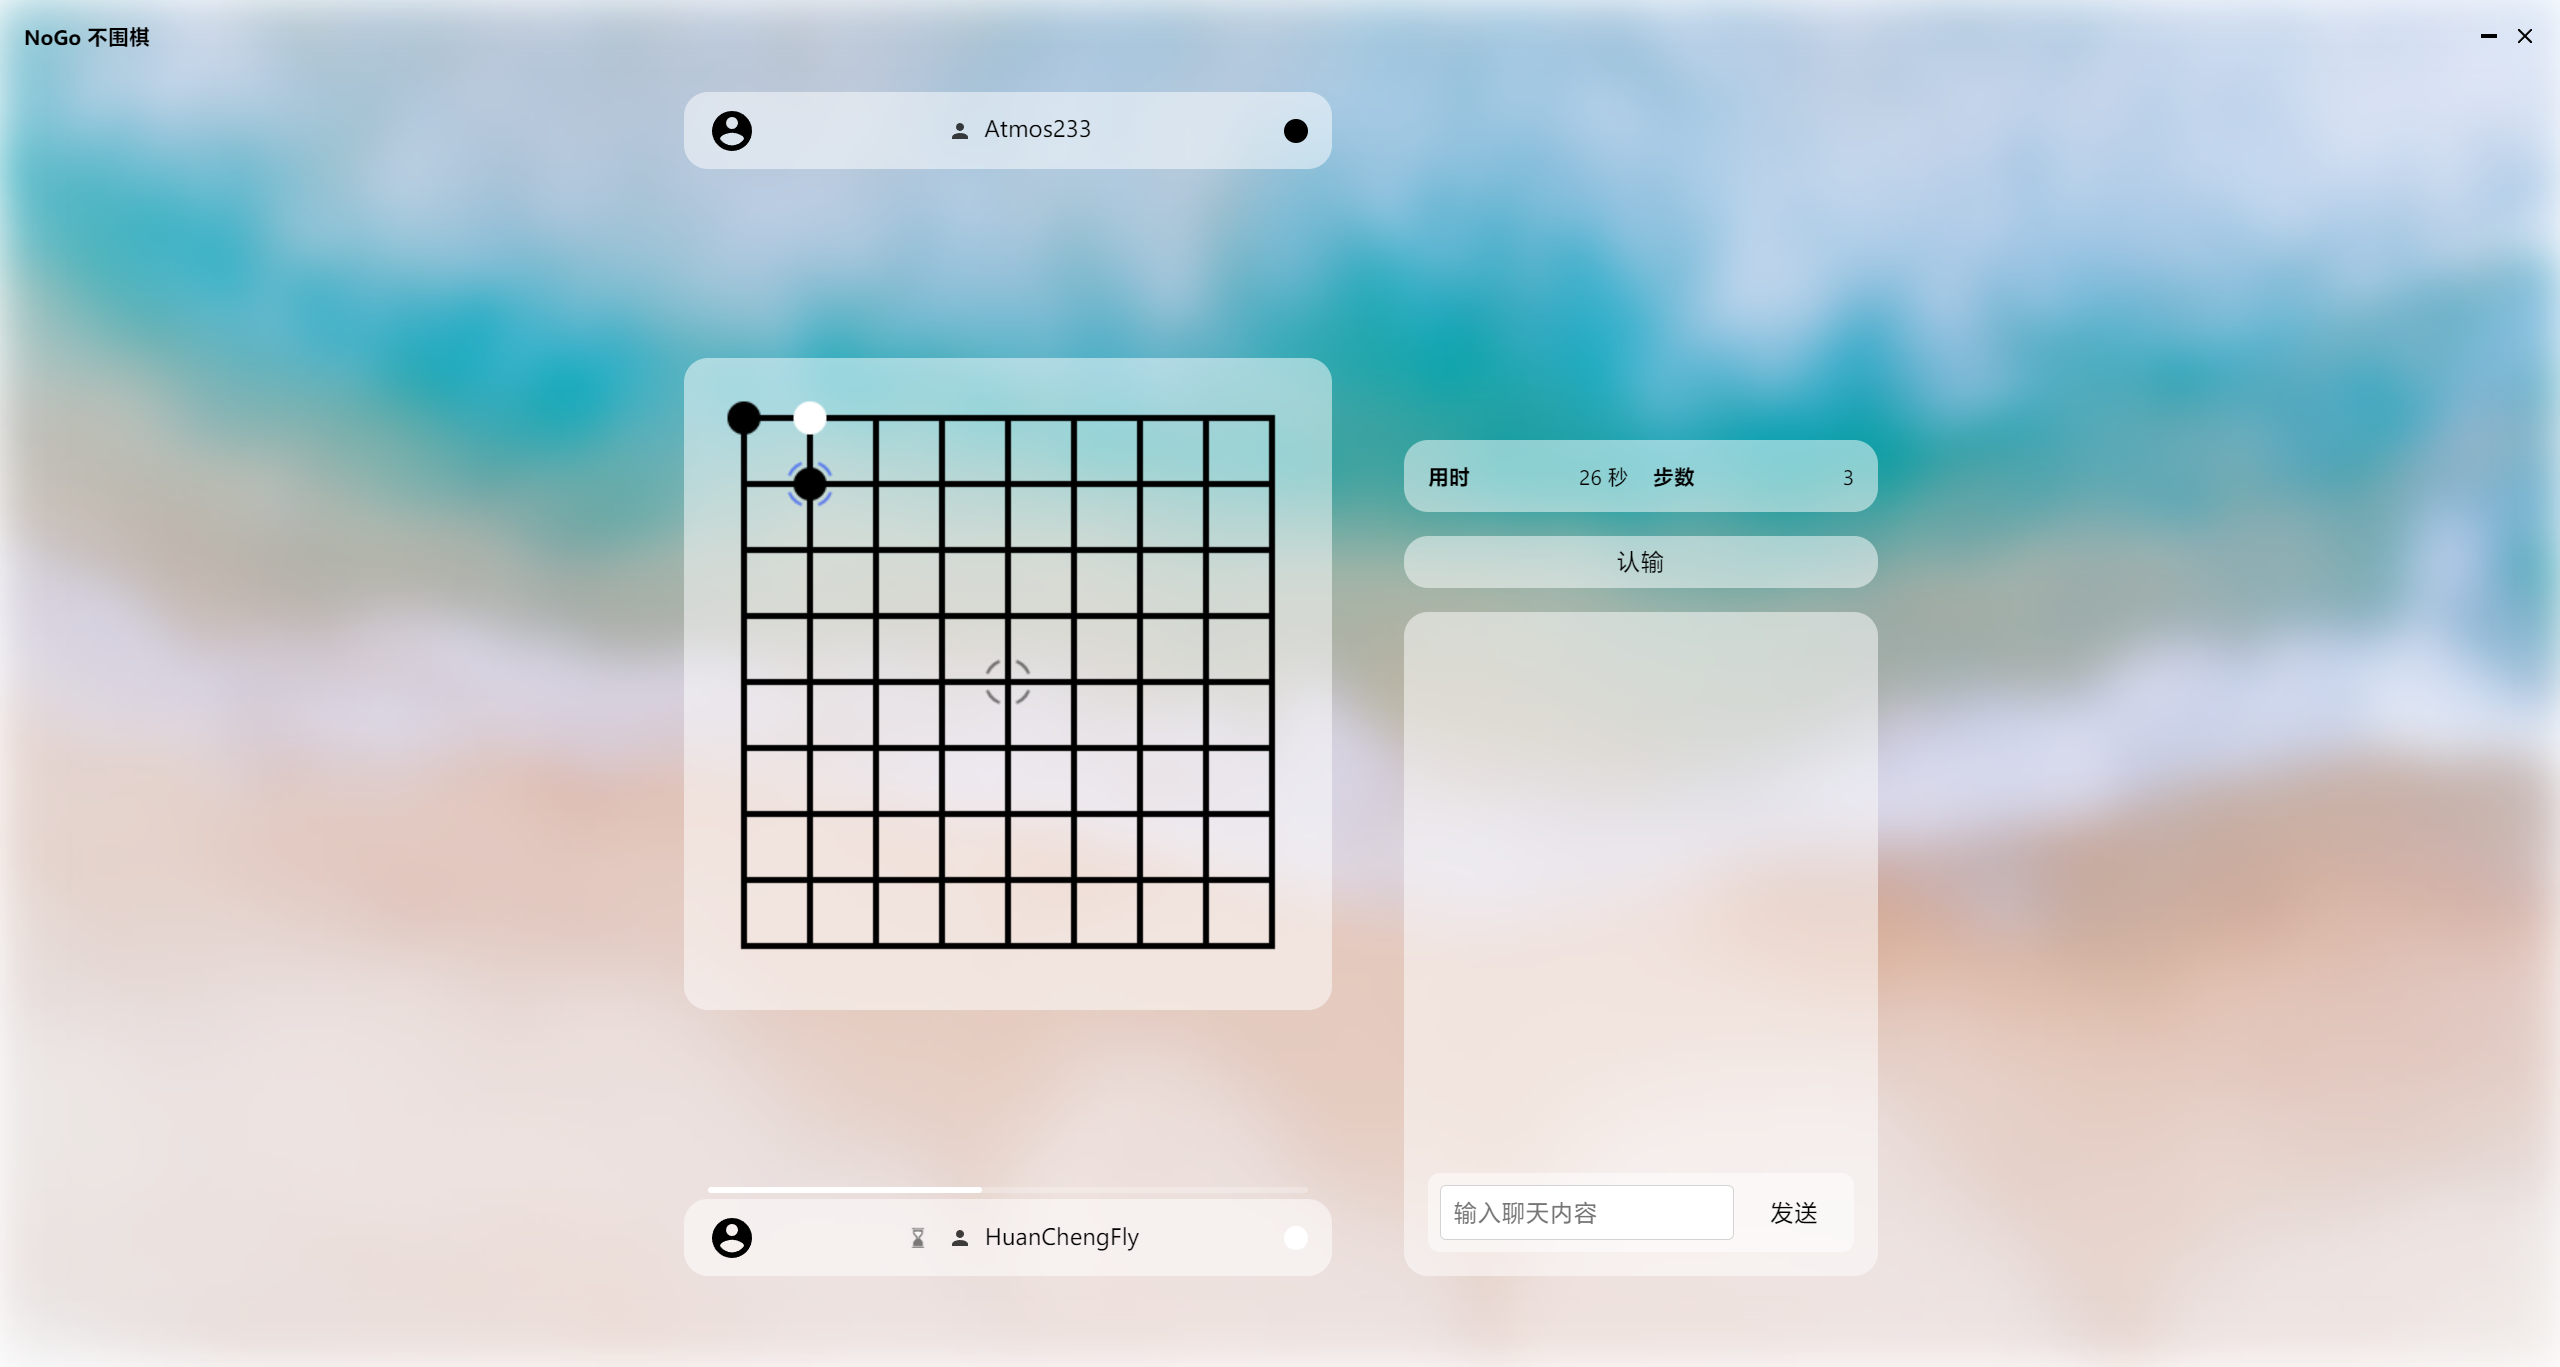
\includegraphics[width=11cm]{Images/OnlineGame.png}
	\caption{联机对局}
\end{figure}
\section{游戏逻辑}

在游戏逻辑方面,我们已经实现了总览中所列的大部分功能,并不再赘述。这里仅对几个尚未完成的部分进行简要说明。\par
我们已经在后端实现了对局记录的保存和复现的相关逻辑。根据编码直接复现最终局面较为容易。但考虑到*附加任务1*和*附加任务2*的要求,我们认为在第三阶段再实现完整的对局复现功能更为合理。因此,我们将在第三阶段完成这项工作。\par

关于多路棋盘功能,由于在实现棋盘类时我们将棋盘的大小作为一个\mintinline{C++}|constexpr|变量\footnote{见 \href{https://github.com/The-Goo-Goo-Gang/nogo-backend/blob/main/rule.hpp\#L37}{\url{nogo-backend/rule.hpp\#L37}}},因此我们在接下来的开发中可以比较方便的将其修改为类的模板参数,从而在后端支持多路棋盘。同时,前端的棋盘组件已经支持了任意大小棋盘的渲染。因此,我们在第三阶段可以较为容易地实现多路棋盘。\par
\section{工程实践}
\subsection{自动构建}
我们使用了 GitHub Actions 来实现自动构建。\par
通过编写 GitHub Actions 的配置文件\footnote{见 \href{https://github.com/The-Goo-Goo-Gang/nogo-backend/blob/main/.github/workflows/xmake.yml}{\url{nogo-backend/.github/workflows/xmake.yml}}},我们实现了自动在 Windows 上的 MSVC、在 Windows 上的 MinGW 和在 Ubuntu 上的 g++ 三种环境下分别进行编译测试。这样,我们就可以在每次提交代码后或有新的 Pull Request 时自动进行编译,以保证代码的可用性。这极大的方便了我们的团队协作,避免了合并代码时可能出现的由于合并冲突导致的编译失败。同时也提高了代码的可移植性。\par
\subsection{测试}

我们使用了 Google Test 来进行单元测试。Google Test是由 Google 开发的 C++ 测试和模拟框架,旨在编写独立、可重复、可组织、可移植、可扩展的测试。\par
在测试中,我们使用了TEST宏来定义一个测试用例。其中,我们创建了一个表示服务器进程的\mintinline{C++}|ServerProcess|对象,并利用 RAII 原则,在测试开始时启动nogo_server程序,并在测试结束时自动终止。
接着,我们创建了两个\mintinline{C++}|Session|对象,分别表示连接到不同端口的TCP连接的会话。通过这两个客户端,我们交替地向服务器发送消息。
最后,我们分别比较了两个客户端接收到的消息与预期的消息是否匹配,以确保服务器的消息处理功能正常运行。

\subsection{日志}
为实现日志功能,我们采用了 spdlog 这一轻量级的 C++11 日志管理库。spdlog 只包含头文件,使用起来非常方便,相比于 glog 有更多的优势。
利用 spdlog 提供的接口,我们编写了一些辅助代码\footnote{见 \href{https://github.com/The-Goo-Goo-Gang/nogo-backend/blob/main/log.hpp}{\url{nogo-backend/log.hpp}}},使得我们可以轻松地将日志同时输出到控制台和按照不同的日志等级分别存储到多个文件中。
例如,下面的代码可以将一条信息级别的日志输出到控制台,并保存到 info.log 文件中,
同时附上玩家的数据:\par 
\begin{center} 
	\mintinline{C++}|logger->info(“player data:{}”, player.to_string());| 
\end{center} \par

在整个项目中,我们广泛地使用了 spdlog 来记录日志。无论是接收、发送、解析信息,还是进行关键的逻辑处理和异常处理,我们都会通过日志来记录程序的运行状态和可能出现的问题。这样做有助于我们及时发现和修复 bug,并在小组联机时快速定位问题所在。\par

\section{展望}
在第三阶段,我们计划完成以下几个任务:
\begin{itemize}
	\item 实现对局复现和多路棋盘
	\item 实现 AI
	\item 完成部分附加任务
	\item 完善自动化测试
	\item 完善文档、注释
\end{itemize}
\section{小组分工}
	\item[\textbf{李知非}] 主要负责项目总体架构设计和后端开发工作\\
	 在第二阶段重新设计了部分架构,实现了游戏逻辑部分的关键功能,参与了联机部分的底层开发和自动化测试的编写;对实验报告进行了全面优化。 
	\item[\textbf{彭文博}] 主要负责 UI 设计和前端开发工作,同时参与后端开发工作\\
	 在第二阶段具体实现了联机部分并优化了前端用户界面,参与了游戏逻辑部分的开发;主持了实验报告的撰写。
	\item[\textbf{魏子洪}] 主要负责测试与文档编写工作,参与前后端开发工作\\
	 在第二阶段实现了日志功能,主导编写了自动化测试脚本,参与了联机部分和游戏逻辑部分的开发;对实验报告进行了审阅。
\end{description}
\section{致谢}
感谢孙亚辉老师在课程中提供的指导与帮助,使我们收获宝贵经验,掌握编程原理。\par
感谢潘俊达助教在项目中给予我们的大力支持,使我们拥有发挥创意、自由探索的机会。\par
感谢王卓冉助教在项目中给予我们指点和建议,使我们迸发对本项目的深入思考。\par

同时,感谢赵培宇同学利用宝贵的时间帮助我们测试程序,并且发现了一个会导致部分电脑上无法运行的严重问题。\par
\appendix
\section{附录}
\subsection{相关链接}
\begin{itemize}
	\item 后端 Repo:\href{https://github.com/The-Goo-Goo-Gang/nogo-backend}{The-Goo-Goo-Gang/nogo-backend}
	\item 前端 Repo:\href{https://github.com/The-Goo-Goo-Gang/nogo-frontend}{The-Goo-Goo-Gang/nogo-frontend}
\end{itemize}
\subsection{关于DDL}
\begin{enumerate}
	\item 程设大作业DDL是5月9日是怎么回事呢?程设大作业相信大家都很熟悉,但是程设大作业DDL是5月9日是怎么回事呢,下面就让小编带大家一起了解吧。\\程设大作业DDL是5月9日,其实就是5月6日开始做,大家可能会很惊讶程设大作业怎么会DDL是5月9日呢?但事实就是这样,小编也感到非常惊讶。
	\item 你说得对,但是《不围棋》是由《程序设计\uppercase\expandafter{\romannumeral2}》自主研发的一款大作业,中间忘了,后面忘了,方便面忘了,牛肉面忘了,高斯面忘了,双侧曲面忘了
\end{enumerate}
\end{document}